\subsection{Optimal parameters choice}
Inside the `Diagonalize $h$' step in figure \ref{fig:pseudocode}, the execution of the GCG algorithm is performed, using the current iteration's single-particle Hamiltonian as the matrix to diagonalize and the previous iteration's orbitals as the initial guess. This is the main computational bottleneck of the code, where a correct choice of the execution parameters can drastically reduce execution times.
The paramters that need to be chosen carefully are essentially the inverse power step tolerance and the number of maximum GCG iterations.
\subsubsection{Inverse power step tolerance}
The first parameter to be tuned is the tolerance on the CG solution of the system \begin{equation}
    AW = \Lambda X
\end{equation}
in algorithm \ref{alg:mod_gcg}, where $A$ is actually the single-particle Hamiltonian $h$.
When the CG residual $AW -  X\Lambda$ is smaller than the tolerance, the procedure stops and outputs the $W$ block.
\\In figure \ref{fig:conv_tol}, the relative absolute error of the total energy is calculated against a reference benchmark value (details in the results chapter \ref{chap:res_sph}), for different values of the CG tolerance. It's clear that at least a tolerance of $10^{-3}$ is needed for good convergence, while tolerances $\ge 10^{-4}$ stop offering increasing returns, rendering a choice between $10^{-4}$ and $10^{-5}$ an optimal one.
\begin{figure}[H]
    \centering
    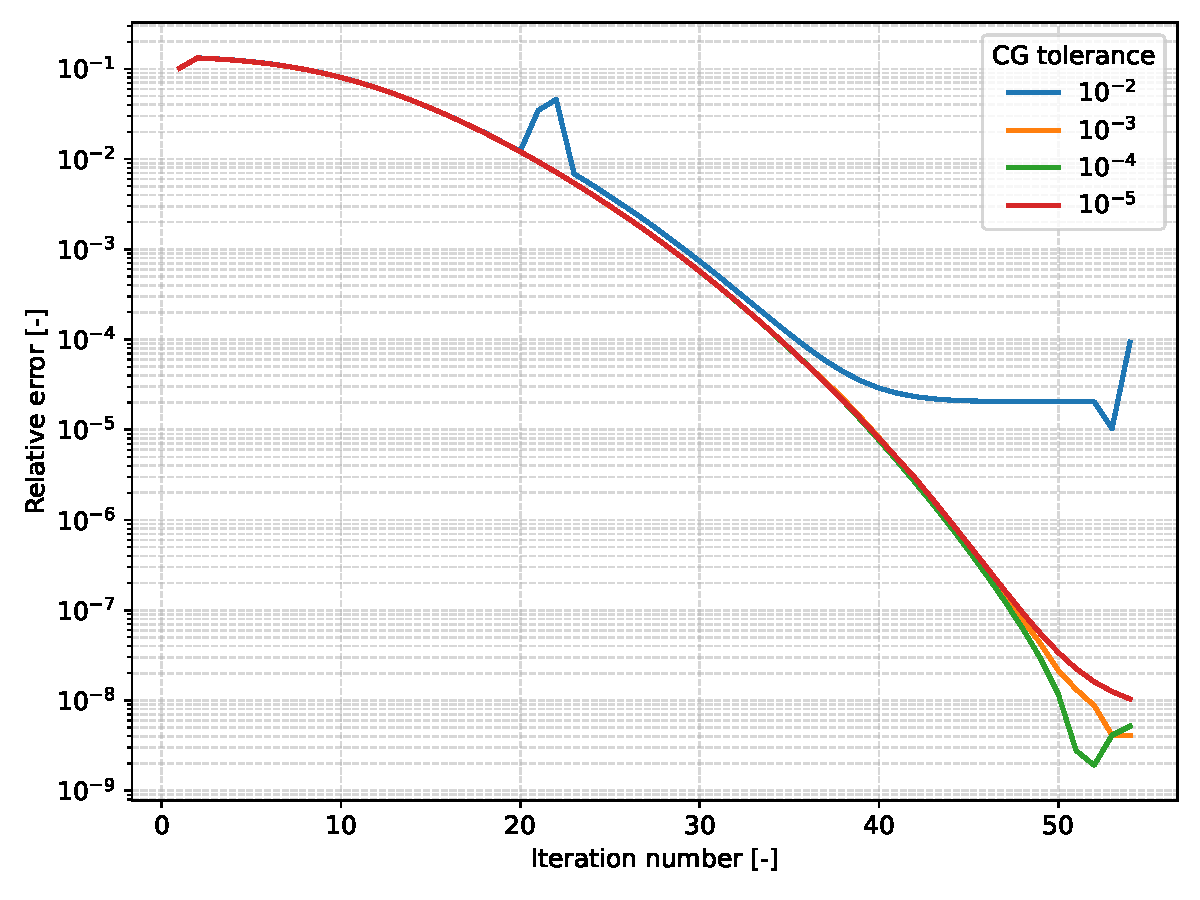
\includegraphics[width=0.9\textwidth]{Images/conv_tol.pdf}
    \caption{HF calculation convergence with varying CG tolerance for $^{16}$O, box $[-9, 9]$ fm, step size $0.3$ fm.} 
    \label{fig:conv_tol}
\end{figure}
\subsubsection{Inner GCG iterations}
The number of inner GCG maximum iterations, here named `inverse power steps' to avoid confusion, is slightly more nuanced than the CG tolerance. The algorithm converges to the true eigenpairs as the power steps are performed, so one could think that a higher number of steps would bring to HF convergence faster, since the precision on the eigenvalues increases, but this is not the case.
\\In figures \ref{fig:conv_steps_o} and \ref{fig:conv_steps_mg}, the convergence of the HF calculation is plotted for different number of steps, respectively, for the spherical nucleus $^{16}$O and the deformed nucleus $^{24}$Mg. 
\begin{figure}[H]
    \centering
    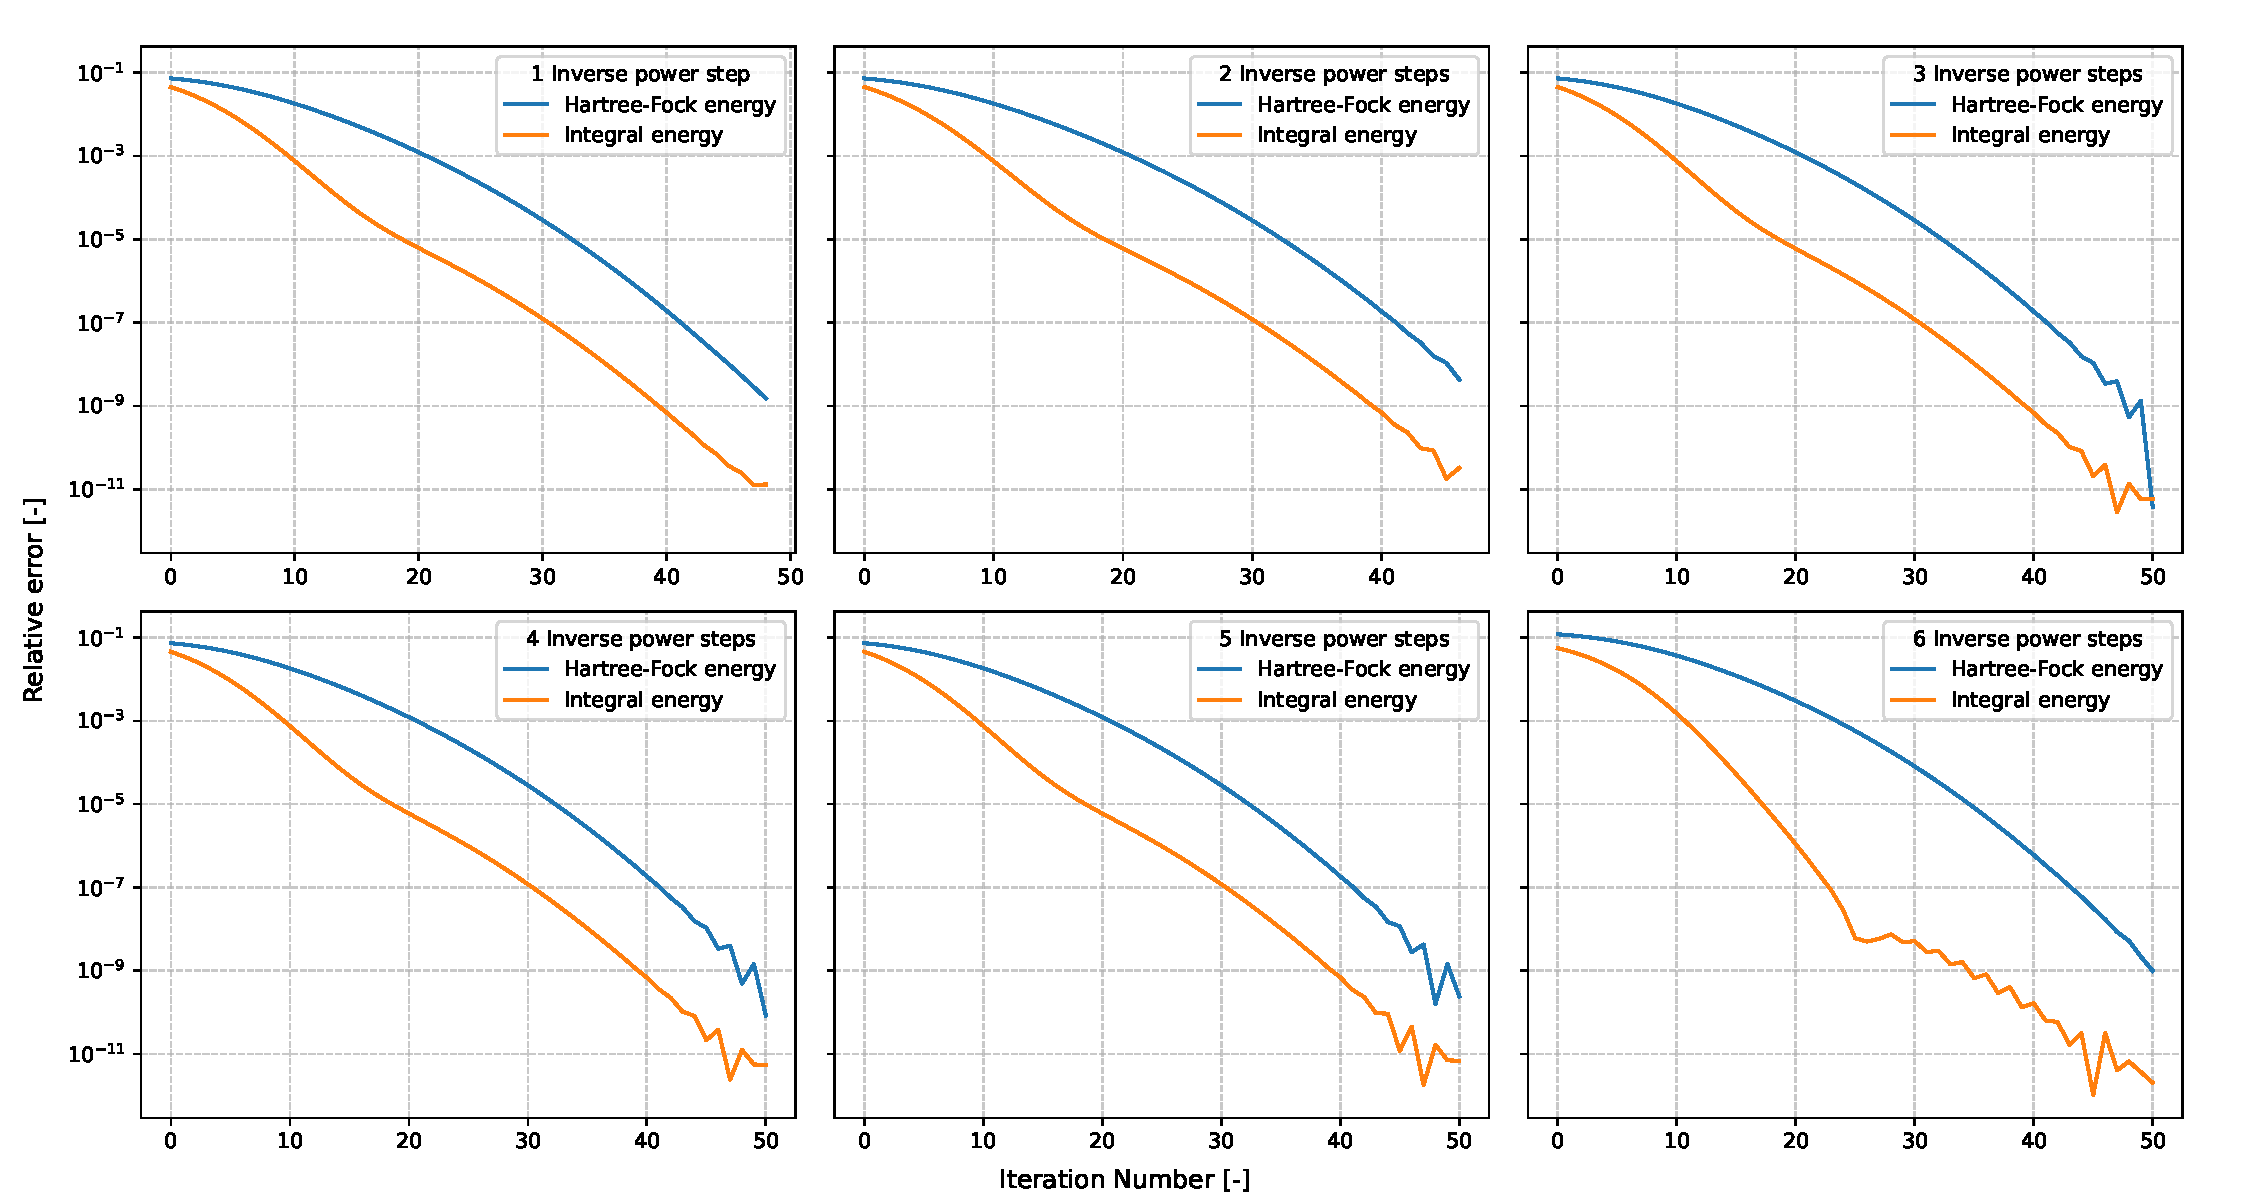
\includegraphics[width=1.0\textwidth]{Images/conv_steps_o.pdf}
    \caption{HF calculation convergence with varying number of inverse power steps for $^{16}$O, box $[-9, 9]$ fm, step size $0.3$ fm.}
    \label{fig:conv_steps_o}
\end{figure}
\begin{figure}[H]
    \centering
    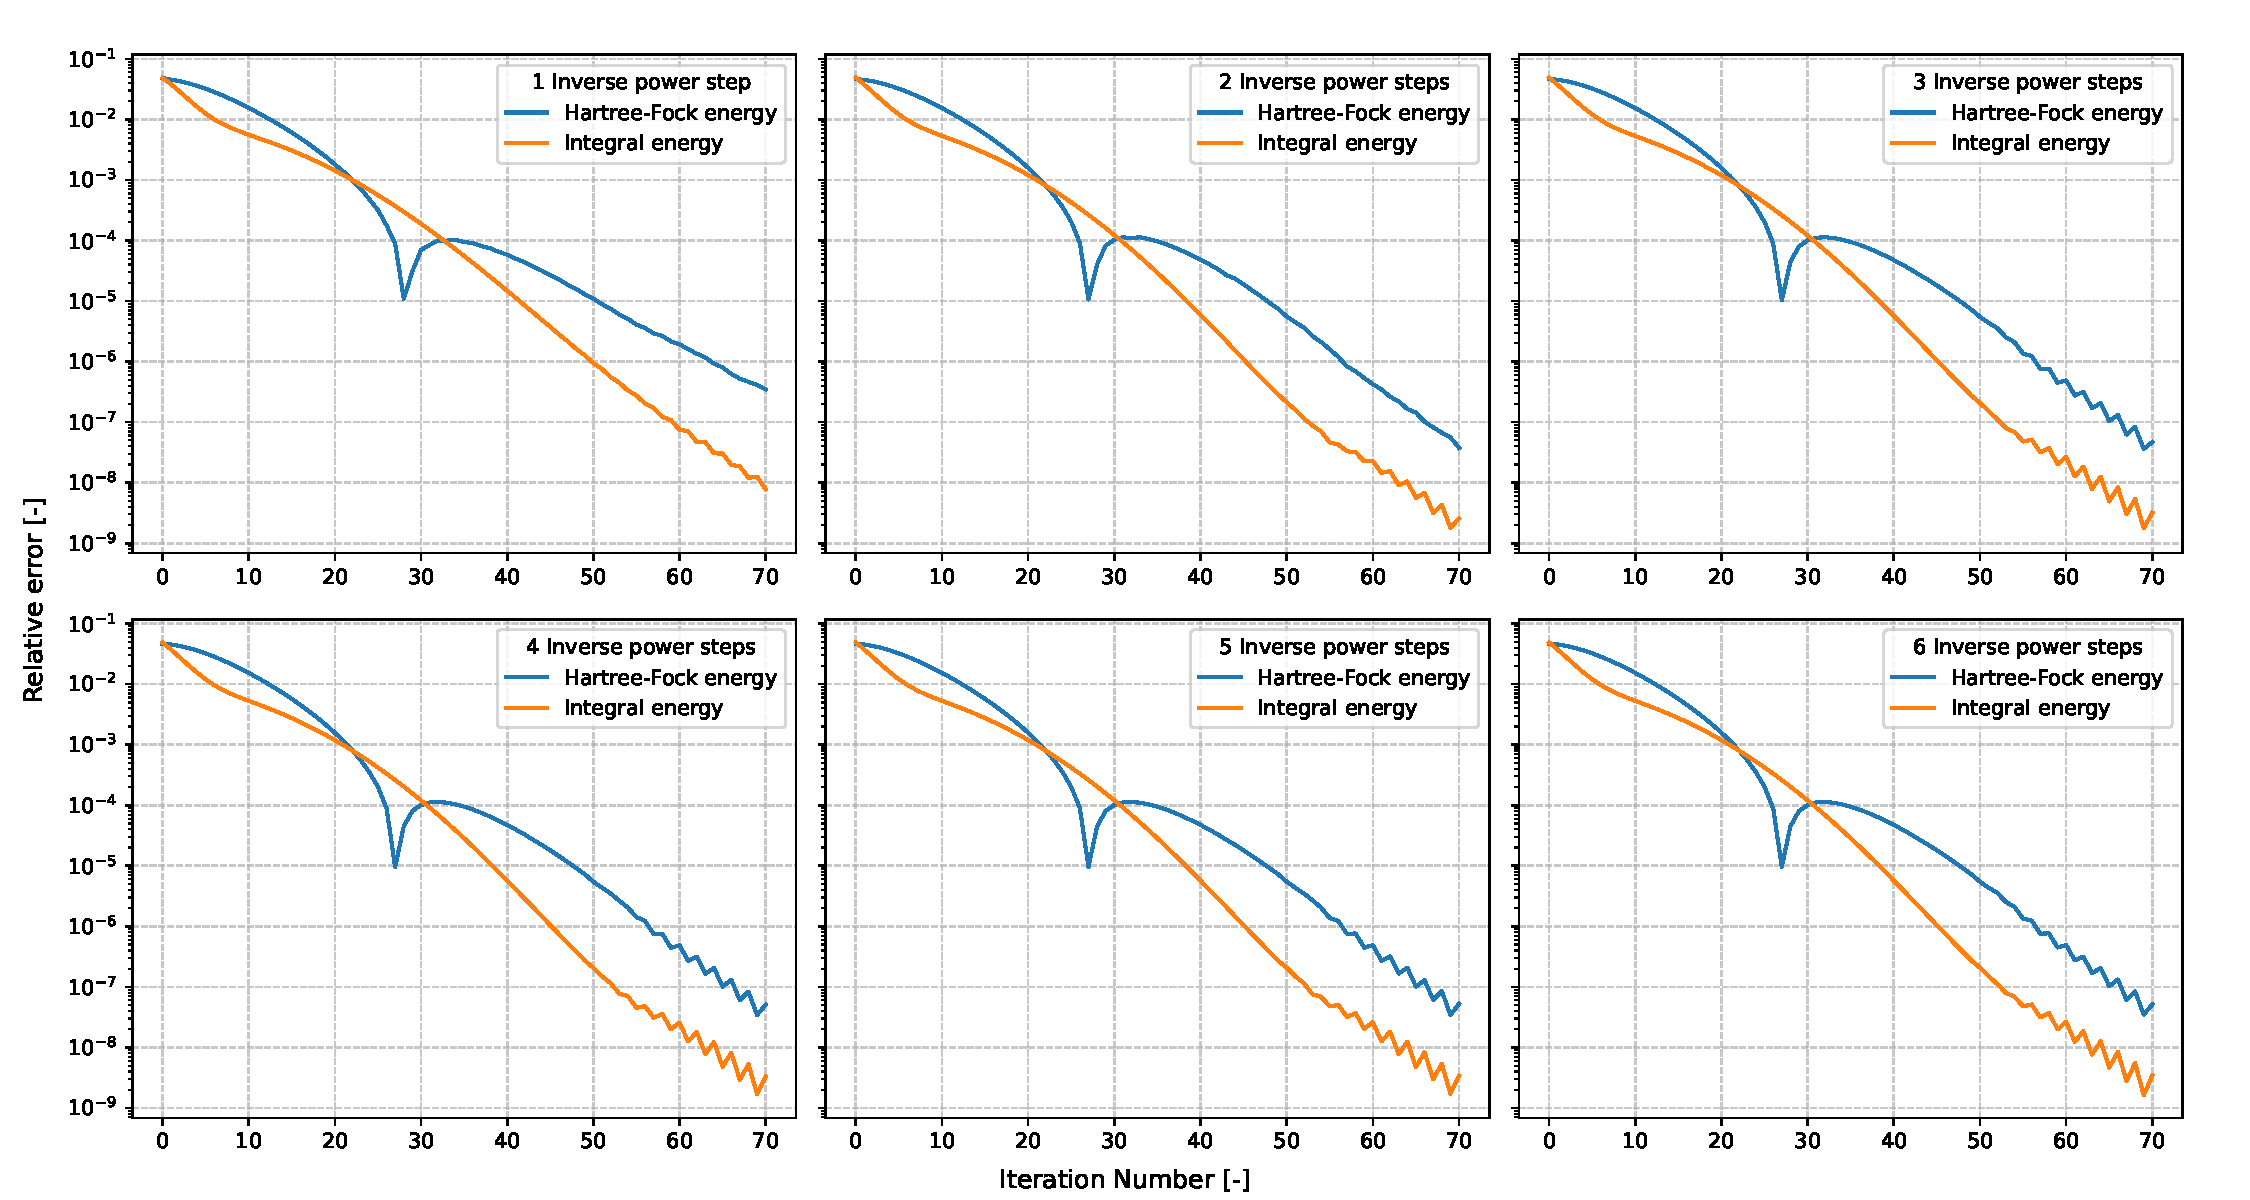
\includegraphics[width=1.0\textwidth]{Images/conv_steps.pdf}
    \caption{HF calculation convergence with varying number of inverse power steps for the deformed nucleus $^{24}$Mg, box $[-10, 10]$ fm, step size $0.33$ fm.}
    \label{fig:conv_steps_mg}
\end{figure}
It's evident that in both cases, a steps number greater than $3$ leads to oscillating behaviour near convergence, without accelerating it, while in the case of the spherical nucleus, just one step is enough to quickly, and reliably reach convergence. In any case, it's clear that delaying the inverse power steps to later HF iterations is safer in terms of stability.
\\This counter intuitive behavior is likely due to the fact that at each HF iteration the hamiltonian changes and a great number of steps leads to solutions too biased towards the current matrix eigenpairs, at the expense of the next iteration; however, in the case of deformed nuclei, due to sharp shape changes at the start of the calculation, just one step may not be enough to sustain the pace at which the Hamiltonian changes, hence the quicker convergence with more steps.



